\documentclass{article}

\usepackage[utf8]{inputenc}
\usepackage[spanish, mexico]{babel}
\usepackage[export]{adjustbox}
\usepackage[shortlabels, inline]{enumitem}
\usepackage{hyperref, amsmath, xcolor, tikz, listings, capt-of}

\usetikzlibrary{shapes.geometric, arrows}

%\usepackage{showframe}
 


\title{ \includegraphics[scale=0.6, right]{itesm_logo}
	    \\[4em] 
        Sistemas Conexionistas y Evolutivos
        \\[2em]
        Tarea completa: incendios forestales
        \\[1em]
        }
\author{ \vspace*{\fill} ---- \qquad\small ---- \\[1em] }

\date{ \vspace*{\fill} \today, Puebla.}


\begin{document}
\maketitle
\newpage

Se presenta el proyecto de clasificación de incendios forestales,
que contiene instrumentos para:
\begin{enumerate*}[1)]
\item extracción de vectores de características de imágenes,
\item entrenamiento de un clasificador,
\item clasificación de imágenes.
\end{enumerate*} 

El proyecto provee la ejecutable \verb|wick|, la cual está descrita en este documento.


\section{Extracción de características}
El proceso de partición de las imágenes en regiones y las características usadas, ya fueron descritas en el reporte del \emph{1"er parcial}.
Aquí solamente se discutirá el uso de \verb|wick| para generación de una base de características.

\medskip
\noindent
Uso: \verb|wick arff <source> <target>|, donde 
\begin{itemize}[leftmargin=9em]
\item[\texttt{<source>}] es paso a la carpeta con imágenes a procesar;
\item[\texttt{<target>}] es paso al archivo ``*.arff'' que será escrito.
\end{itemize}

Extrae las características, preguntando al usuario \emph{la clase} de cada región en
una interfaz gráfica.

\medskip
\noindent
Opciones:
\begin{itemize}[align=left]
\item[\texttt{--save-regions <value>}] --- Guardar las regiones en la carpeta \verb|<value>|.
                                           Se guardan como: nombre de imagen original +
                                           posición de la región + clase asignada.
\item[\texttt{--name} o \texttt{-n <value>}] --- Establecer el nombre de la relación a \verb|<value>|, que va ser escrito en el archivo  ``*.arff'' \verb|<target>|.
\item[\texttt{--no-class} o \texttt{-?}] --- En lugar de preguntar las clases al usuario, asigna todos las clases como desconocidas ``?''.
\end{itemize}

\noindent
Ejemplo:

\verb|wick arff ~/Pictures/wildfire fire1.arff --save-regions reports|

\subsection{Clases utilizadas}

Las clases utilizadas fueron revisadas desde el reporte del 1"er parcial:
\begin{itemize}[leftmargin=6em]
\item[\texttt{Fire}]    --- la región contiene fuego abierto;
\item[\texttt{Smoke}]   --- la región contiene humo, pero no fuego abierto;
\item[\texttt{Neither}] --- la región no contiene ningún signo de incendio;
\item[\texttt{Ignore}]  --- la región no debe ser utilizado para el aprendizaje.
\end{itemize}

\begin{figure}[!h]
    \centering
    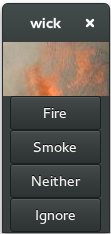
\includegraphics{wick-arff}
    \caption{La interfaz gráfica, preguntando al usuario la clase de la región demostrada.}
\end{figure}

\section{Entrenamiento}

El proceso de entrenamiento usa como clasificador un \emph{perceptron de múltiples capas},
en Weka --- la clase \verb|MultilayerPerceptron|.
Internamente, se usa un \verb|FilteredClassifier|, el cual pre-procesa las instancias,
usadas para el entrenamiento. Se usan los siguientes dos filtros:
\begin{itemize}[leftmargin=10em]
\item[\texttt{NominalToBinary}] para transformar las etiquetas de clase a valores numéricos,
                                con los cuales ya puede trabajar una red neuronal;
\item[\texttt{RemoveWithValues}] para remover las instancias, marcadas con la clase \verb|Ignore|.
\end{itemize}


\bigskip
\noindent

Uso: \verb|wick model <source> <target>|, donde
\begin{itemize}[leftmargin=9em]
\item[\texttt{<source>}] es paso al archivo ``*.arff'' con los datos de entrenamiento;
\item[\texttt{<target>}] es paso al archivo ``*.model'' que será escrito.
\end{itemize}

Entrena un modelo de perceptron multi-capa y lo escribe en formato de Weka.

\medskip
\noindent
Opciones:
\begin{itemize}[align=left]
\item[\texttt{--validate} o \texttt{-x <value>}] --- Correr una validación cruzada con el número 
                                                     de particiones \verb|<value>|, después de 
                                                     haber entrenado el modelo. 
                                                     Se imprime en la consola.
\item[\texttt{--x-report <value>}] --- Guardar en reporte de validación en el 
                                       archivo \verb|<value>|.
\item[\texttt{--options} u \texttt{-o <value>}] --- Establecer los parámetros de entrenamiento
                                                    de la red. Para evitar la mal interpretación
                                                    de los parámetros como argumentos de
                                                    \verb|wick|, incluye los argumentos entre
                                                    \verb|""|.
\item[\texttt{--tikz-confusion <value>}] --- Genera un diagrama de confusión, basado en los
                                             resultados de la validación cruzada.
                                             Se escribe en el archivo \verb|value| en formato
                                             de \emph{Tikz} -- un paquete para \LaTeX.
\end{itemize}

\noindent
Ejemplo:

\begin{verbatim}
    wick model fire1.arff fire1.model\
         -x 4 --x-report report.log\
         -o "-L 0.1 -M 0.5 -H t,a -N 500"\
         --tikz-confusion confusion.tikz.tex

\end{verbatim}

%\begin{figure}[!h]
\begin{center}
    \lstinputlisting[language={}, basicstyle=\footnotesize, frame=none, basewidth=0.46em]
                    {report.log} 
    \captionof{figure}{Reporte de validación cruzada.}
\end{center}
%\end{figure}
%\begin{figure}[!h]
\begin{center}
    \resizebox{\textwidth}{!}{ \begin{tikzpicture}[>=triangle 60]
\tikzset{ class/.style={align=center, minimum height=4ex,text width=6em,
                        draw, circle} };
\def\psize{15cm}

\node[draw=none,regular polygon,minimum size=\psize,regular polygon sides=4] (poly) {};

\node[class] (N1) at (poly.corner 1) { \textbf{Fire} \\ 410 of 516\\$\approx \mathbf{79\%}$ };
\node[class] (N2) at (poly.corner 2) { \textbf{Ignore} \\ 0 of 0\\$\approx \mathbf{0\%}$ };
\node[class] (N3) at (poly.corner 3) { \textbf{Neither} \\ 762 of 869\\$\approx \mathbf{87\%}$ };
\node[class] (N4) at (poly.corner 4) { \textbf{Smoke} \\ 481 of 575\\$\approx \mathbf{83\%}$ };

\begin{scope}[draw=red, text=red]
\draw (N1) edge [->, bend left] node[label=left:{$0\%$}]{} (N2);
\draw (N1) edge [->, bend right] node[label=left:{$12\%$}]{} (N3);
\draw (N1) edge [->, bend left] node[label=left:{$7\%$}]{} (N4);
\end{scope}

\begin{scope}[draw=black, text=black]
\draw (N2) edge [->, bend left] node[label=left:{$0\%$}]{} (N1);
\draw (N2) edge [->, bend left] node[label=left:{$0\%$}]{} (N3);
\draw (N2) edge [->, bend right] node[label=left:{$0\%$}]{} (N4);
\end{scope}

\begin{scope}[draw=green!50!black, text=green!50!black]
\draw (N3) edge [->, bend right] node[label=left:{$6\%$}]{} (N1);
\draw (N3) edge [->, bend left] node[label=left:{$0\%$}]{} (N2);
\draw (N3) edge [->, bend left] node[label=left:{$5\%$}]{} (N4);
\end{scope}

\begin{scope}[draw=orange!50!black, text=orange!50!black]
\draw (N4) edge [->, bend left] node[label=left:{$6\%$}]{} (N1);
\draw (N4) edge [->, bend right] node[label=left:{$0\%$}]{} (N2);
\draw (N4) edge [->, bend left] node[label=left:{$10\%$}]{} (N3);
\end{scope}

\end{tikzpicture} }
    \captionof{figure}{Un diagrama de confusión, generado por \texttt{wick}.}
\end{center}
%\end{figure}


\section{Clasificación}

La clasificación de una imagen se hace a partir de clasificaciones de sus regiones.
Se usa el modelo, entrenado en sección 2.
El proceso de partición de imágenes en regiones es el mismo de la sección 1.

\medskip
\noindent
Uso: \verb|wick class <source> <target>|, donde
\begin{itemize}[leftmargin=9em]
\item[\texttt{<source>}] es paso al archivo ``*.model'' con el modelo entrenado;
\item[\texttt{<target>}] es paso a la carpeta con imágenes a clasificar.
\end{itemize}

Procesa cada imagen y reporta si contiene signos de incendio y las regiones dónde estos se encuentran.

\medskip
\noindent
Opciones:
\begin{itemize}[align=left]
\item[\texttt{--gui} o \texttt{-G}] --- Mostrar los resultados de clasificación en la interfaz gráfica.
\item[\texttt{--par <value>}] --- (Experimental) Ejecutar en paralelo con \verb|<value>| ejecutadores asíncronos.
\end{itemize}

\noindent
Ejemplo: \verb|wick class fire1.model ~/Pictures/wildfire -G|



\subsection{Resultados de clasificación}

Ejemplos de la interfaz gráfica de clasificación:  
{\color{red} fuego}, {\color{orange} humo} , {\color{green} ninguno}.
\begin{center}
    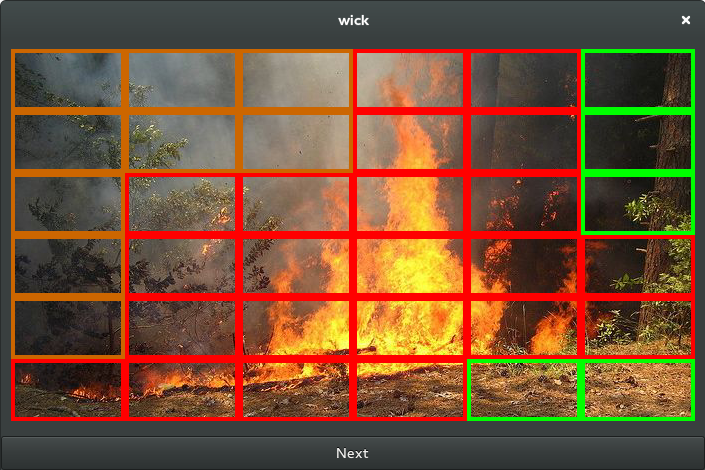
\includegraphics[width=\textwidth]{wick-class-01}
    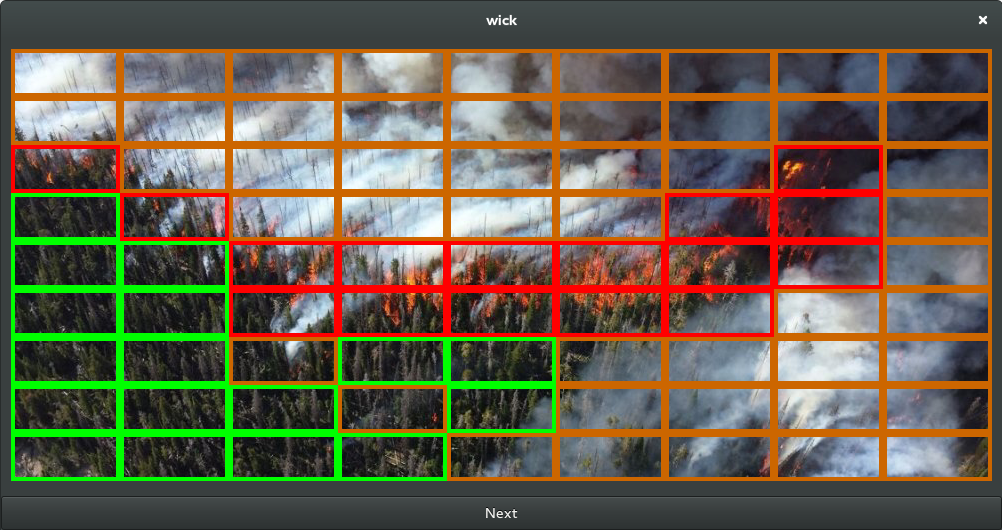
\includegraphics[width=\textwidth]{wick-class-02}
    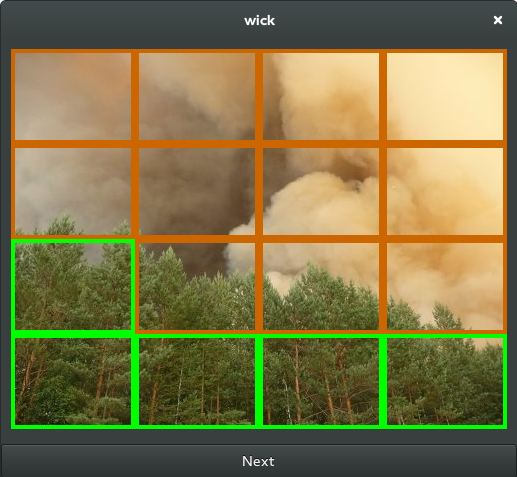
\includegraphics[width=\textwidth]{wick-class-03}
    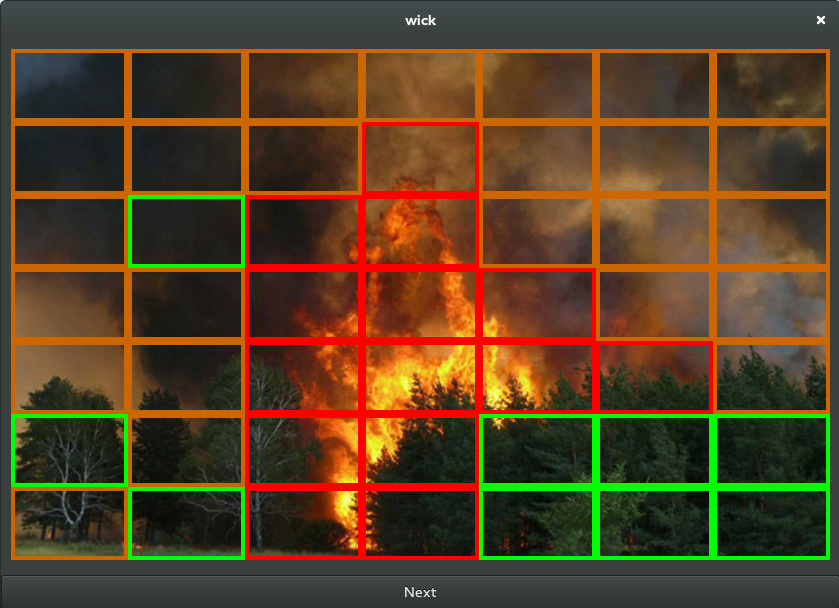
\includegraphics[width=\textwidth]{wick-class-04}
    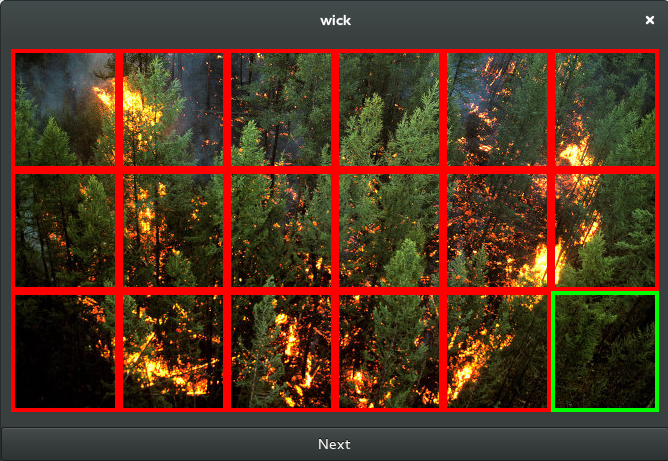
\includegraphics[width=\textwidth]{wick-class-05}
    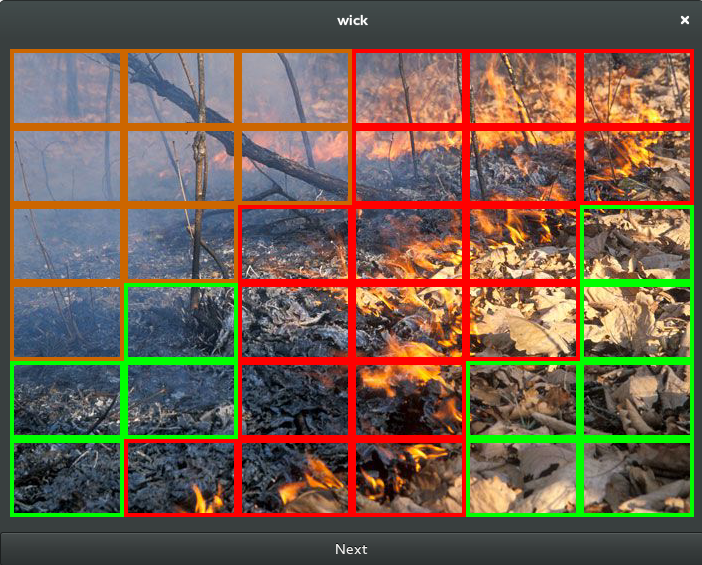
\includegraphics[width=\textwidth]{wick-class-06}
    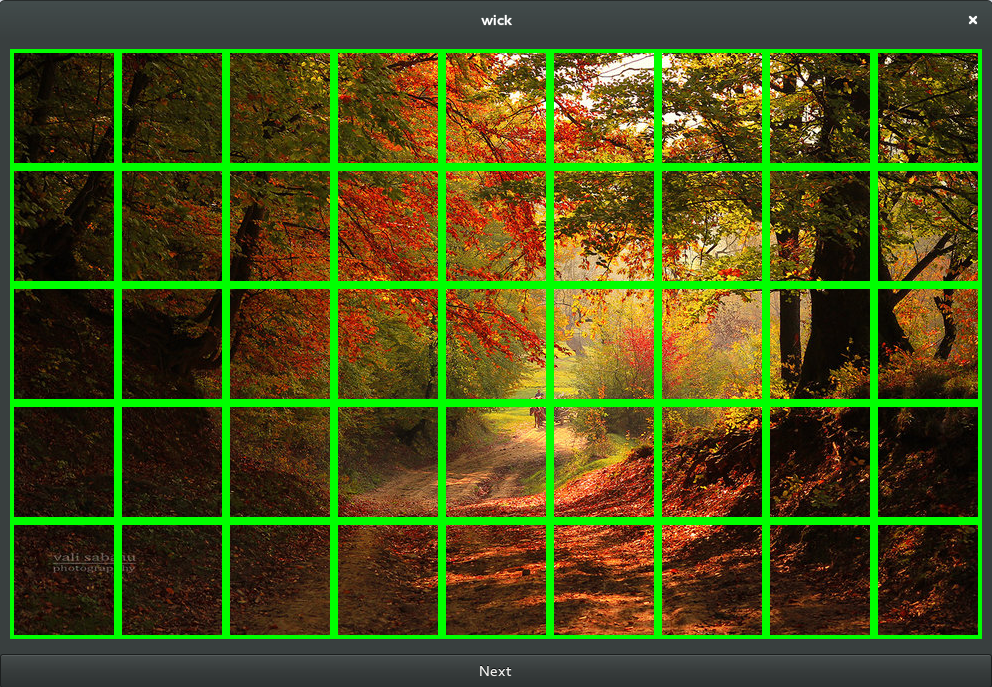
\includegraphics[width=\textwidth]{wick-class-07}
\end{center}

\newpage
\lstinputlisting[language={}, frame=none, basicstyle=\footnotesize, breaklines=true]
                {classify.log} 

\end{document}